\chapter{Introdução} \label{Introducao}

No cenário atual da manufatura, marcado pela competitividade, pela busca por eficiência operacional e pela necessidade de respostas rápidas às demandas produtivas, a digitalização de processos tornou-se relevante para a gestão industrial. A transformação digital está associada ao crescimento e à sobrevivência das organizações, pois envolve o uso de tecnologias digitais para modificar produtos, processos e aspectos organizacionais, promovendo competitividade e geração de valor \cite[p.~1]{terra2022}. No ambiente industrial, essa transformação contribui para o aumento da produtividade, o aprimoramento do controle da qualidade e a ampliação da flexibilidade operacional \cite[p.~1]{ribeiro2026}.

A partir dessa perspectiva, a digitalização não deve ser compreendida apenas como a substituição de registros físicos por meios digitais, mas como uma forma de reorganizar informações e rotinas para apoiar a gestão e a tomada de decisão. A transformação digital nas organizações provoca mudanças em processos produtivos, estrutura organizacional, modelos de negócio, competências, cultura e liderança, desde que alinhada à estratégia corporativa \cite[p.~57]{murici2022}.

Nesse contexto, as plataformas \textit{low code} apresentam-se como recursos capazes de apoiar iniciativas de digitalização ao facilitar o desenvolvimento rápido de aplicações voltadas às necessidades operacionais da organização. Essas plataformas reduzem a dependência de programação manual tradicional, pois utilizam interfaces visuais e elementos pré-configurados para a criação de aplicações, permitindo maior agilidade, menor complexidade e maior participação dos usuários ligados ao negócio no desenvolvimento de soluções digitais \cite[p.~2]{sanchis2020}.

A relevância dessas plataformas pode ser observada na pesquisa apresentada por \citeonline[p.~3]{sanchis2020}, baseada em um levantamento realizado com mais de 3.300 profissionais de tecnologia da informação em diferentes continentes. Conforme apresentado na Figura~\ref{fig:motivos-low-code}, 66\% dos respondentes indicaram a aceleração da transformação digital e o aumento da capacidade de resposta às demandas do negócio como os principais motivos para o uso de plataformas \textit{low code}. Além disso, 45\% destacaram a redução da dependência de competências técnicas difíceis de contratar.

Esses resultados são relevantes para este estudo porque aproximam o uso de plataformas \textit{low code} das necessidades práticas observadas em ambientes industriais, nos quais a agilidade no desenvolvimento de soluções, a redução de registros manuais e a maior disponibilidade de informações podem contribuir para a melhoria da gestão operacional. Dessa forma, a adoção desse tipo de ferramenta pode ser compreendida como uma alternativa para apoiar iniciativas de digitalização em processos produtivos.

Assim, este estudo concentra-se na análise da digitalização de processos industriais em uma empresa de manufatura, considerando a aplicação de uma ferramenta \textit{low code} como apoio à substituição de registros manuais por registros digitais, à organização das informações e à melhoria da gestão das informações no ambiente produtivo.


\begin{figure}[htb]
\caption{\label{fig:motivos-low-code}Principais razões para adoção de plataformas de desenvolvimento \textit{low code}}
\centering
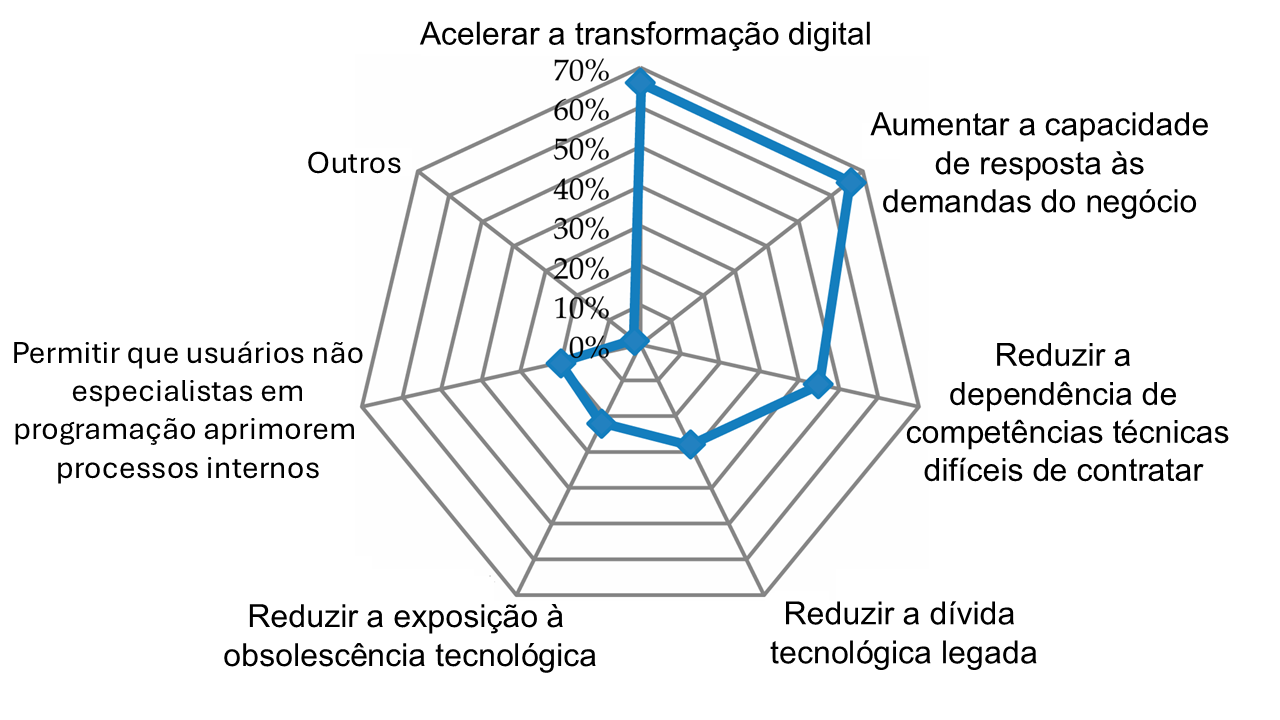
\includegraphics[width=0.78\textwidth]{Figuras/figura_motivos_low_code_pt.png}
\legend{Fonte: Adaptado de \citeonline[p.~3]{sanchis2020}.}
\end{figure}


% \dangersign[3ex] {\color{red}
% Não se esqueça de modificar o número de páginas antes da introdução (sem contar a capa)!
% No arquivo Monografia.tex altere a seguinte linha (no lugar de 14 coloque o valor contado de páginas): 
% $\backslash setcounter\{page\}\{11\} $% Inserir aqui o número de páginas antes da introdução menos a capa
% }


\section{Justificativa}

A manufatura contemporânea está inserida em um cenário de forte competitividade, no qual a eficiência operacional, a qualidade e a rapidez no acesso às informações tornaram-se fatores importantes para a gestão dos processos produtivos. Nesse contexto, a transformação digital passa a ter papel relevante, pois envolve o uso de tecnologias digitais para modificar produtos, processos e aspectos organizacionais, contribuindo para a competitividade e a geração de valor \cite[p.~1]{terra2022}. No ambiente industrial, essas mudanças também se relacionam ao aumento da produtividade, ao aprimoramento do controle da qualidade e à ampliação da flexibilidade operacional \cite[p.~1]{ribeiro2026}.

A justificativa deste trabalho está relacionada à necessidade de compreender como o uso de soluções digitais pode apoiar a organização e o acompanhamento de informações em processos industriais. Em rotinas produtivas, registros manuais ou pouco integrados podem dificultar a padronização dos dados, o acesso às informações e a análise das atividades realizadas. Além disso, a transformação digital nas organizações envolve alterações em processos produtivos, estrutura organizacional, competências, cultura e formas de gestão, desde que esteja alinhada à estratégia corporativa \cite[p.~57]{murici2022}. Dessa forma, analisar um caso real de manufatura permite observar como a digitalização pode contribuir para tornar as informações operacionais mais acessíveis e úteis à gestão.

Nesse cenário, as ferramentas \textit{low code} mostram-se adequadas ao tema deste estudo por possibilitarem maior agilidade na criação de aplicações e menor dependência de programação manual tradicional. Segundo Sanchis et al. \cite[p.~2]{sanchis2020}, essas plataformas utilizam interfaces visuais e elementos pré-configurados, permitindo maior participação de usuários ligados ao negócio no desenvolvimento de soluções digitais. Assim, este trabalho se justifica por analisar a aplicação de uma ferramenta \textit{low code} na digitalização de processos industriais, contribuindo para a compreensão de alternativas mais ágeis e adaptáveis para apoiar a gestão das informações no ambiente produtivo.



\section{Objetivos}

\subsection{\textit{Objetivo geral}}

O presente trabalho apresenta como objetivo geral analisar a digitalização de dois processos industriais em uma empresa de manufatura por meio da aplicação de uma ferramenta \textit{\textit{low code}}.

\subsection{\textit{Objetivos específicos}}

\begin{itemize}
\item Caracterizar os processos industriais analisados, considerando suas formas de registro, acompanhamento e organização das informações antes da digitalização.

\item Descrever a aplicação da ferramenta \textit{low code} nos processos estudados, observando sua utilização no contexto da empresa de manufatura.

\item Analisar as mudanças percebidas nos processos após a digitalização, considerando a acessibilidade, a padronização e a organização das informações.

\item Avaliar, a partir do estudo de caso, as contribuições da ferramenta \textit{low code} para o acompanhamento das rotinas operacionais e para a gestão das informações no ambiente produtivo.

\end{itemize}

\section{Organização do Texto}

No Capítulo 2 deste trabalho é apresentada a fundamentação teórica, abordando os principais conceitos relacionados à transformação digital, digitalização de processos industriais, manufatura e ferramentas \textit{low code}. No Capítulo 3 são descritos os procedimentos metodológicos utilizados para a realização do estudo de caso, considerando a caracterização da pesquisa, o ambiente analisado e as etapas adotadas para a análise dos processos. No Capítulo 4 são apresentados e discutidos os resultados obtidos a partir da análise da digitalização dos processos industriais estudados. Por fim, no Capítulo 5, são apresentadas as considerações finais do trabalho, destacando os principais resultados, limitações e sugestões para trabalhos futuros.


%Sugestões para estrutura da monografia:

% \begin{enumerate}[label=(\alph*)]
%   \item Introdução
%   \item Referencial Teórico (ou Revisão Bibliográfica)
%   \item Materiais e Métodos (ou Metodologia)
%   \item Resultados e Discussões
%   \item Conclusão (ou Considerações Finais)
%   \item Referências
% \end{enumerate}








